\documentclass[answers]{exam}
\usepackage{amsmath, amsfonts, amssymb, amstext, amscd, amsthm, makeidx,
graphicx, hyperref, url, enumerate}

\title{Problem Set 2, EE 150/CS 148a, Winter 2025}
\author{TAs: Andrew Zabelo and Armeet Jatyani}
\date{}

\begin{document}
\maketitle

\begin{questions}

\question[10] Dropout

\begin{parts}
\part[5] Dropout Equivalence to $\ell_2$ Regularization

Show that OLS Regression with dropout is equivalent to Ridge Regression by
proving that the expected squared loss with dropout is of the following form:
\[ E[L(w)] = \|y - f(p)Xw\|^2 + g(p)\|\Gamma w\|^2 \]
where $f(p)$ and $g(p)$ are functions of $p$, and $\Gamma$ is a diagonal matrix
with the standard deviations of features in data matrix $X$.

\begin{solution}
The expected OLS loss is 

\[
\mathbb{E}[\mathcal{L}(w)] = ||y - \mathbb{E}[Xw]||^2 + \mathbb{E}[||\mathbb{E}[Xw] - Xw||^2]
.\] 

In dropout, we zero out each weight randomly. Thus, the predictions of a OLS
model with dropout can be written as 

\[
    \hat{y} = XMw
,\] 

where $M$ is a mask matrix of size $D \times D$ where $D$ is the dimension of
the weights. $M$ is an indentity matrix with the $i$-th diagonal value being 0
if $w_{i}$ is zeroed out for dropout. Thus, the expected loss for OLS with
dropout is

\[
\mathbb{E}[\mathcal{L}(w)] = ||y - \mathbb{E}[XMw]||^2 + \mathbb{E}[||\mathbb{E}[XMw] - XMw||^2]
.\] 

We know $\mathbb{E}[M]=\frac{1}{1-p}I$, where $I$ is a $D \times D$ identity
matrix. This is because each value along the diagonal is an independent
Bernoulli random variable with probability of $p$ of being 0 and $1-p$ to be 1.

Computing the bias via linearity of expectation,

\[
||y - \mathbb{E}[XMw]||^2 = ||y - X\mathbb{E}[M]w||^2 = \left|\left|y - (1-p)Xw \right|\right|^2
.\] 

To compute the variance, we first substitute the expected value of the
prediction:

\[
\sigma^2 = \mathbb{E}[||\mathbb{E}[XMw] - XMw||^2] = \mathbb{E}[||(1-p)Xw - XMw||^2]
.\] 

Now, we expand the expression inside the outer expected value using its
quadratic form:

\begin{align*}
\sigma^2 &= ||(1-p)Xw - XMw||^2 \\ 
&= ((1-p)Xw)^T((1-p)Xw) - 2 ((1-p)Xw)^{T}(XMw) + (XMw)^{T}(XMw) \\ 
&= (1-p)^2w^{T}X^{T}Xw - 2(1-p)w^{T}X^{T}XMw + w^{T}M^{T}X^{T}XMw
.\end{align*}

Computing the expected value,

\begin{align*}
\sigma^2 &= \mathbb{E}\left[(1-p)^2w^{T}X^{T}Xw - 2(1-p)w^{T}X^{T}XMw + w^{T}M^{T}X^{T}XMw\right] \\
         &= (1-p)^2w^{T}X^{T}Xw -2(1-p)w^{T}X^{T}X\mathbb{E}[M]w + \mathbb{E}[w^{T}M^{T}X^{T}XMw] \\ 
         &= (1-p)^2w^{T}X^{T}Xw -2(1-p)^2w^{T}X^{T}Xw + (1-p)w^{T}X^{T}Xw
.\end{align*}

In the above computation, the last expected value in the second line is
simplifies as such because the expected value of the square of a Bernoulli r.v.
is the expected value of just the regular Bernoulli r.v.

We know that $\Gamma$, the standard deviation matrix, is the diagonal matrix
with elements being the square root of the sum of the variances in each column
of covariance matrix of $X$. Thus, $||w^{T}X^{T}Xw|| = ||\Gamma w||^2$.
Substituting this in,

\[
\sigma^2 
= (1-p)^2 ||\Gamma w|^2 - 2(1-p)^2||\Gamma w|^2 + (1-p)||\Gamma w|^2 
= p(1-p)||\Gamma w||^2
.\] 

Thus, we have 

\[ 
E[L(w)] = \|y - f(p)Xw\|^2 + g(p)\|\Gamma w\|^2 ,
\]

where $f(p) = 1-p$ and $g(p)=p(1-p)$
\end{solution}

\part[5] Dropout Code
Create a copy of the Dropout Colab Notebook and rename it to Dropout \{first name last name\}.ipynb. Follow the instructions to generate a Loss vs. Dropout Rate plot.

\begin{solution}
\href{https://colab.research.google.com/drive/1sBnaC6m1BGGmdqYaBcLRK2_5Ey0d2d4H?usp=sharing}{colab link}
\end{solution}
\end{parts}

\question[10] Batch Normalization

\begin{parts}
\part[5] BatchNorm Backpropagation
Given $\frac{\partial L}{\partial Y}$, derive expressions for:
\begin{itemize}
    \item $\frac{\partial L}{\partial \beta}$
    \item $\frac{\partial L}{\partial \gamma}$
    \item $\frac{\partial L}{\partial X}$
\end{itemize}

\begin{solution}
\[
Y_{ij} = \gamma_{j}\hat{X}_{ij} + \beta_{j} 
\implies Y_{i} = \gamma^{T} \odot \hat{X}_{i} + \beta
\implies \frac{\partial Y_{i}}{\partial \beta^{T}} = 1 
\implies \frac{\partial \mathcal{L}}{\partial \beta} = 
\sum_{i=1}^{N} \left( \frac{\partial \mathcal{L}}{\partial Y_{i}}  \right)^{T}
\] 
\[
Y_{ij} = \gamma_{j}\hat{X}_{ij} + \beta_{j} 
\implies Y_{i} = \gamma^{T} \odot \hat{X}_{i} + \beta
\implies \frac{\partial Y_{i}}{\partial \gamma^{T}} = \hat{X}_{i}
\implies \frac{\partial \mathcal{L}}{\partial \gamma} = 
\sum_{i=1}^{N} \left( \frac{\partial \mathcal{L}}{\partial Y_{i}} \odot \hat{X}_{i} \right)^{T}
\] 
\[
Y_{ij} = \gamma_{j}\hat{X}_{ij} + \beta_{j} 
\implies Y_{i} = \gamma^{T} \odot X_{i} + \beta
\implies \frac{\partial Y_{i}}{\partial \hat{X}_{i}} = \gamma^{T}
\implies \frac{\partial \mathcal{L}}{\partial \hat{X}} = 
\frac{\partial \mathcal{L}}{\partial Y} \odot \begin{bmatrix} 
\gamma^{T} \\ 
\vdots \\ 
\gamma^{T}
\end{bmatrix}
\] 

Now, we know that $\hat{X}_{ij} = (X_{ij} - \mu_{j}) / \sqrt{\sigma^2_{j} 
+ \epsilon}$. Since $\mu_{j},\sigma^2_{j}$ are both functions of $X_{ij}$,
we need to apply quotient rule and chain rule:

\[
\frac{\partial \hat{X}_{ij}}{\partial X_{ij}} = 
\frac{s_{j}(X_{ij}-\mu_{j})' - (X_{ij} - \mu_{j})s'_{j}}{s_{j}^2}
.\] 

Here, $s_{j}$ is $\sqrt{\sigma^2_{j} + \epsilon}$. Computing the gradients, 
we have

\begin{align*}
\mu'_{j} &= \frac{1}{N} \\ 
s'_{j} &= \frac{1}{2\sqrt{\sigma^2_{j}+\epsilon}} \cdot \frac{\partial}{\partial X_{ij}} (\sigma^2_{j} + \epsilon) \\ 
&= \frac{1}{2s_{j}} \cdot \frac{\partial}{\partial X_{ij}} \cdot \frac{1}{N} \cdot \sum_{k=1}^{N} (X_{kj} - \mu_{j})^2 \\
&= \frac{1}{2s_{j}} \cdot \frac{2}{N} \cdot \sum_{k=1}^{N} (X_{kj} - \mu_{j}) \cdot \frac{\partial}{\partial X_{ij}} (X_{kj}-\mu_{j}) \\
&= \frac{1}{2s_{j}} \cdot \frac{2}{N} \cdot \left( X_{ij} - \mu_{j} + \sum_{k=1}^{N} (X_{kj} - \mu_{j}) \cdot \left( -\frac{1}{N} \right) \right) \\
&= \frac{1}{Ns_{j}} \cdot \left( X_{ij} - \mu_{j}\right).
\end{align*}

In the above calculation for $s'_{j}$, the summation for $k=1,\ldots,N$ cancels
out because the sums of the difference with a mean is 0. The extra 
$X_{ij} - \mu_{j}$ term comes from the fact that when $k=i$, the partial
derivative of $(X_{ij} - \mu_{j})$ w.r.t. $X_{ij}$ is $1 - \mu'_{j}$.

Thus, for $\hat{X}_{ij}$, the derivative is 

\begin{align*}
\frac{\partial \hat{X}_{ij}}{\partial X_{ij}} &= 
\frac{s_{j}(1 - \frac{1}{N}) - (X_{ij} - \mu_{j}) \cdot \frac{1}{Ns_{j}} (X_{ij} - \mu_{j})}{s_{j}^2} \\
&= \frac{1}{s_{j}} - \frac{1 + \hat{X}_{ij}^2}{Ns_{j}}
.\end{align*}

However, we still have to account for the role $X_{ij}$ plays in $\hat{X}_{kj},
k\neq i$ since $ X_{ij}$ is used in $\mu_{j}, s_{j}$ for those terms as well.

\begin{align*}
\frac{\partial \hat{X}_{kj}}{\partial X_{ij}} &= \frac{s_{j}(X_{kj}-\mu_{j})' - (X_{kj} - \mu_{j})s'_{j}}{s_{j}^2} \\ 
&= \frac{s_{j}\left( -\frac{1}{N} \right) - (X_{kj}-\mu_{j}) \cdot \frac{1}{Ns_{j}}(X_{ij}-\mu_{j})}{s_{j}^2} \\
&= -\frac{1 + \hat{X}_{kj}\hat{X}_{ij}}{Ns_{j}}
.\end{align*}

Combining the derivatives from $\hat{X}_{kj}$ and $\hat{X}_{ij}$ with the values
of $\frac{\partial \mathcal{L}}{\partial \hat{X}_{ij}}$,

\[
\frac{\partial \mathcal{L}}{\partial X_{ij}} = 
\frac{1}{s_{j}} \cdot \frac{\partial \mathcal{L}}{\partial \hat{X}_{ij}} 
- \frac{1}{Ns_{j}} \sum_{k=1}^{N} \frac{\partial \mathcal{L}}{\partial \hat{X}_{kj}} 
-  \frac{\hat{X}_{ij}\sum_{k=1}^{N}\hat{X}_{kj} \cdot \frac{\partial \mathcal{L}}{\partial \hat{X}_{kj}}}{Ns_{j}}
.\] 

Not sure if the TA reading this is looking for the OG Batchnorm paper
derivation, so here's the comparision: essentially, in the sum above, the first
term is the derivative that comes from the contribution of $X_{ij}$ to every
$\hat{X}_{ij}$, the second term is from the contribution of $X_{ij}$ to every
time the mean is used to compute an element in column $j$ for $\hat{X}$, and the
last term is the contribution of $X_{ij}$ to every time the variance is used to
compute an element in column $j$ in $\hat{X}$.  

To put this into matrix form (as a product of a Jacobian of sorts with the
matrix of $\frac{\partial L}{\partial \hat{X}}$, which we will now denote $D$),
notice that the matrix corresponding to the first term is $\frac{1}{s_{j}} \odot
(ID)$, where $I$ is the identity matrix, the second term can be written as
$-\frac{1}{Ns_{j}}\odot (\textbf{1}D)$, where $\textbf{1}$ is the matrix of
all ones, and the last term corresponds to $\frac{1}{Ns_{j}} \odot\hat{X} \odot
\left( \textbf{1} \cdot (\hat{X} \odot D)\right)$. Thus, our gradient for the
input is

\[
\frac{\partial \mathcal{L}}{\partial X} = 
\frac{1}{s_{j}} \odot (I \frac{\partial \mathcal{L}}{\partial Y} \odot [\gamma^{T}] ) 
- \frac{1}{Ns_{j}}\odot(\textbf{1} \frac{\partial \mathcal{L}}{\partial Y} \odot [\gamma^{T}]) 
- \frac{1}{Ns_{j}} \odot \hat{X} \odot \left( \textbf{1} (\hat{X}\odot \frac{\partial \mathcal{L}}{\partial Y} \odot [\gamma^{T}]) \right) 
.\] 

In the equation above, $[\gamma^{T}]$ is the $N \times D$ matrix with its rows being
$\gamma^{T}$.
\end{solution}

\part[5] Batch Normalization Code
Implement BatchNorm from scratch and verify that your implementation matches PyTorch’s built-in BatchNorm function.

\begin{solution}
\href{https://colab.research.google.com/drive/1fvWNh_8h5VLk5Xgeo1WXGn6VHQGhb66g?usp=sharing}{colab link}

Holy shit it actually works I didn't think my formula was right since it was
different from the batchnorm paper's.
\end{solution}
\end{parts}

\question[15] Layer Normalization

\begin{parts}
\part[5] LayerNorm Backpropagation
Given $\frac{\partial L}{\partial Y}$, derive expressions for:
\begin{itemize}
    \item $\frac{\partial L}{\partial \beta}$
    \item $\frac{\partial L}{\partial \gamma}$
    \item $\frac{\partial L}{\partial X}$
\end{itemize}

\begin{solution}
There's no change for $\beta$ and $\gamma$ since the dimensions for those are
still the same. 

\[
Y_{ij} = \gamma_{j}\hat{X}_{ij} + \beta_{j} 
\implies Y_{i} = \gamma^{T} \odot \hat{X}_{i} + \beta
\implies \frac{\partial Y_{i}}{\partial \beta^{T}} = 1 
\implies \frac{\partial \mathcal{L}}{\partial \beta} = 
\sum_{i=1}^{N} \left( \frac{\partial \mathcal{L}}{\partial Y_{i}}  \right)^{T}
\] 
\[
Y_{ij} = \gamma_{j}\hat{X}_{ij} + \beta_{j} 
\implies Y_{i} = \gamma^{T} \odot \hat{X}_{i} + \beta
\implies \frac{\partial Y_{i}}{\partial \gamma^{T}} = \hat{X}_{i}
\implies \frac{\partial \mathcal{L}}{\partial \gamma} = 
\sum_{i=1}^{N} \left( \frac{\partial \mathcal{L}}{\partial Y_{i}} \odot \hat{X}_{i} \right)^{T}
\] 
\[
Y_{ij} = \gamma_{j}\hat{X}_{ij} + \beta_{j} 
\implies Y_{i} = \gamma^{T} \odot X_{i} + \beta
\implies \frac{\partial Y_{i}}{\partial \hat{X}_{i}} = \gamma^{T}
\implies \frac{\partial \mathcal{L}}{\partial \hat{X}} = 
\frac{\partial \mathcal{L}}{\partial Y} \odot \begin{bmatrix} 
\gamma^{T} \\ 
\vdots \\ 
\gamma^{T}
\end{bmatrix}
\] 

As for $X$, since it's analagous to the transposed version of batchnorm, if we
sum from $j=1\ldots D$, we should have the correct formulas for layernorm
backprop. Notice that we also commute any matrix multiplications since we want
it over the $D$ dimension this time, not the $N$ dimension.

\[
\frac{\partial \mathcal{L}}{\partial X} = 
\frac{1}{s_{i}} \odot (\frac{\partial \mathcal{L}}{\partial Y}I \odot [\gamma^{T}] ) 
- \frac{1}{Ns_{i}}\odot(\frac{\partial \mathcal{L}}{\partial Y} \textbf{1} \odot [\gamma^{T}]) 
- \frac{1}{Ns_{i}} \odot \hat{X} \odot \left( (\hat{X}\odot \frac{\partial \mathcal{L}}{\partial Y} \odot [\gamma^{T}]) \textbf{1} \right) 
.\] 
\end{solution}


\part[5] Layer Normalization Code
Implement LayerNorm from scratch and verify correctness against PyTorch’s
built-in LayerNorm.

\begin{solution}
    \href{https://colab.research.google.com/drive/1iVcwAy4x0Yi_5Zprh3HvZzJjjhYhr73C?usp=sharing}{colab link}
\end{solution}

\part[5] BatchNorm LayerNorm Puzzle
Bob has access to $Y$ from BatchNorm. How many elements in $Z$ (LayerNorm output) does Bob know with certainty if $X$ is symmetric?

\begin{solution}
For any $\gamma, \beta$, all of them. If the matrix is symmetric, then the mean
and variance across the batch and feature dimensions are the same. Thus, the
normalization without the affine transformation across the layer and batch
dimensions are the same. Then, applying the affine transformation doesn't change
anything since the outputs of the normalization are the same.
\end{solution}
\end{parts}

\question[40] Regularization, Optimizers, and Augmentation in MNIST

\begin{parts}
\part[10] Regularization
\begin{enumerate}
\item Plot the distribution of weights of a newly initialized model. Let $X$ be
    a random variable that is the value of a parameter chosen at random from our
    uninitialized model. Write an expression for the PDF of $X$. Why is it
    beneficial for the standard deviation of the initial distribution of a layer
    to decrease as layer width increases?
\item Plot the distribution of weights of a model trained using SGD.
    Qualitatively, what is the new distribution of weights?
\item Now plot the distribution of weights of a model trained using SGD and
    weight decay $0.01$. Qualitatively, what changed about the distribution? In
    theory, why should this help a model’s ability to generalize to unseen data?
\item $\ell_2$ regularization on weights (not to be confused with $\ell_2$
    regularization on model outputs) and weight decay are often used
    interchangeably, but they are in fact distinct methods. Prove that for
    standard SGD, $\ell_2$ regularization and weight decay are equivalent.

Weight decay update: \[ w_{t+1} \leftarrow w_t - (\nabla_w L +
\lambda_{\text{weight decay}} w_t) \]

$\ell_2$ regularized update: \[ w_{t+1} \leftarrow w_t - (\nabla_w L) \] where
\[ L = \lambda_{\ell_2} \sum_{i} w_i^2 \]

\item Use your solution from part (d) to run SGD with $\ell_2$ regularization
    with the $\ell_2$ lambda that would make it equivalent to SGD with weight
    decay $0.01$. How does the distribution of weights compare to part (c)?
\end{enumerate}

\begin{solution}
\href{https://colab.research.google.com/drive/1tJlZ-QLsr9tMvhipsfVXQ-yYTJ757TNL?usp=sharing}{colab}

The distribution of new weights is the sum of multiple uniform distributions.
The pdf is roughly

\[
p(x) \approx \begin{cases}
    0.03 &\quad \text{if } x \in (-0.5, 0.5) \\
    0.14 &\quad \text{if } x \in [-0.1, -0.05] \cup [0.05, 0.1]
\end{cases}
.\] 

It makes sense for the the standard deviation of the initial distribution of a
layer to decrease as layer width increases to make the next layer doesn't have
an insanely high variance/standard deviation. 

The distribution of weights trained with SGD is normal. In theory, this makes
sense since naturally occuring data generally follows a uniform distribution.

$\ell_2$ regularization and and weight decay are the same because the gradient
of the sum of the squares of the weights is just the current weights times 2.
Thus, the $\lambda_{\ell_2} = \frac{1}{2} \lambda_{\text{weight decay}}$. The
distribution of the weights is the same.
\end{solution}

\part[15] Optimizers:
\begin{enumerate}
\item Derive the bias correction term $\frac{1}{1-\beta^t}$ for the Adam
    optimizer and show that it is necessary to un-bias the estimates for the
    first and second moments.
\item Explain why adding an $\ell_2$ regularization penalty to the loss is
    problematic when using SGD with momentum. Discuss its effect when using
    RMSProp and Adam optimizers.
\item Explain how AdamW correctly penalizes weights in contrast with Adam.
\item Run the following and report the validation accuracies. Which two methods
    perform best? Why do the others perform worse?
\begin{itemize}
    \item Adam, default
    \item Adam, $\ell_2$ lambda=0.005
    \item Adam, weight decay=0.01
    \item AdamW, $\ell_2$ lambda=0.005
    \item AdamW, weight decay=0.01
\end{itemize}
\end{enumerate}

\begin{solution}
The formula for the moment are

\begin{align*}
m_{t} &= \beta_1 m_{t-1} + (1 - \beta_1)g_{t} \\
v_{t} &= \beta_2 m_{t-1} + (1 - \beta_2)g_{t}^2 \\
.\end{align*}

Rewriting this non-recursively as a sum of terms,

\begin{align*}
m_{t} &= (1-\beta_1) \sum_{i=1}^{t}\beta_1^{t-i} g_{i}  \\
v_{t} &= (1-\beta_2) \sum_{i=1}^{t}\beta_2^{t-i} g_{i}^2 \\
.\end{align*}

Taking the expecvted value,

\begin{align*}
\mathbb{E}[m_{t}] &= \mathbb{E}\left[(1-\beta_1) \sum_{i=1}^{t}B_1^{t-i} g_{i}\right] \\
\mathbb{E}[v_{t}] &= \mathbb{E}\left[(1-\beta_2) \sum_{i=1}^{t}\beta_2^{t-i} g_{i}^2\right] \\
.\end{align*}

As the model converges, $g_i$ becomes more stable and $g_i \to \mathbb{E}[g]$, 
the expected value becomes

\begin{align*}
\mathbb{E}[m_{t}] &= (1-\beta_1) \sum_{i=1}^{t}B_1^{t-i} \mathbb{E}[g] \\
\mathbb{E}[v_{t}] &= (1-\beta_2) \sum_{i=1}^{t}\beta_2^{t-i} \mathbb{E}[g^2]\\
.\end{align*}

Since we can estimate the expected values related to the gradients as constants,
we can take them out and sum the geometric series:

\begin{align*}
\mathbb{E}[m_{t}] &= (1-\beta_1) \frac{1-\beta_1^{t}}{1-\beta_1} \mathbb{E}[g] \\
&= (1-\beta_1^{t})\mathbb{E}[g] \\
\mathbb{E}[v_{t}] &= (1-\beta_2) \frac{1-\beta_2^{t}}{1-\beta_2} \mathbb{E}[g^2] \\
&= (1-\beta_2^{t})\mathbb{E}[g^2]
.\end{align*}

$m_{t}$ and $v_{t}$ are supposed to be moving averages of the gradient and
gradient squared, but clearly their expected value is biased by a factor of
$(1-\beta_1^{t})$ and $(1-\beta_2^{t})$. Thus, to unbias them, we need to
multiply them by $\frac{1}{1-\beta_1^{t}}$ and $\frac{1}{1-\beta_2^{t}}$.

Adding $\ell_2$ regularization penalty to the loss whne using SGD with momentum,
RMSProp, and Adam is problematic because the penalty term creates a gradient
that is not related to the training error when these optimizers calculate the
moving average for momentum. AdamW correctly penalizes weights because separates
the calculation for weight decay from loss by simply removing a scalar factor of
the weights during the update rule instead of using the $\ell_2$ penalty term.

\href{https://colab.research.google.com/drive/1tJlZ-QLsr9tMvhipsfVXQ-yYTJ757TNL?usp=sharing}{Colab}

Using Adam with no weight decay or regularization worked best, but using AdamW
with weight decay worked the best since AdamW accounts for momentum when using
weight decay. AdamW does this by performing the weight decay updated and the 
momentum update separately, not by backpropagating the weight decay term as a
gradient of the loss. Thus, the gradient from the L2 loss is not factored in
when it computes the momentum.
\end{solution}

\part[15] Data Augmentation: 
\begin{enumerate}
\item Implement methods for common image transformations: rotations, translations, blurring, scaling, shear, and Gaussian noise addition.
\item Display the effects of each augmentation using one example for each digit (0-9). Ensure augmented images remain recognizable.
\item Evaluate augmentation effects on performance:
\begin{itemize}
    \item Train a model on the small dataset and note validation accuracy.
    \item Apply different augmentation strengths and train models to report:
    \begin{itemize}
        \item Augmentation that decreases accuracy by $\leq1\%$.
        \item Augmentation that decreases accuracy by $1-3\%$.
        \item Augmentation that decreases accuracy by $\geq3\%$.
    \end{itemize}
\end{itemize}
\item Investigate rotation range impact by setting $(-180,180)$ and analyze misclassifications via a confusion matrix.
\item Develop a method to randomly apply augmentations to scale the dataset to 50,000 images. Train models and report validation accuracy for:
\begin{itemize}
    \item Small dataset (5,000 images).
    \item Small dataset copied 10 times (50,000 images).
    \item Augmented dataset (50,000 images).
    \item Original dataset (50,000 images).
\end{itemize}
\end{enumerate}

\begin{solution}
\href{https://colab.research.google.com/drive/1tJlZ-QLsr9tMvhipsfVXQ-yYTJ757TNL?usp=sharing}{colab}

\begin{center}
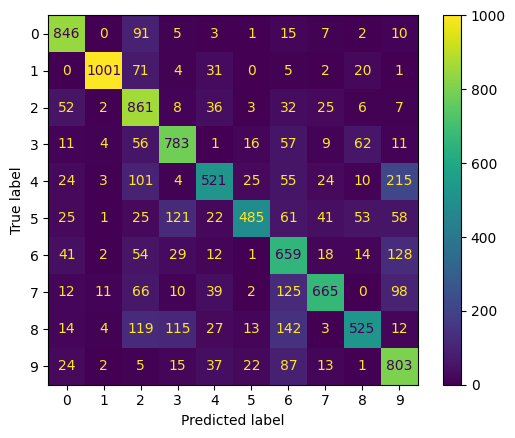
\includegraphics[width=0.8\textwidth]{img/4d.png}
\end{center}

The most misclassified numbers are 4 and 9, with 6 and 9 being the second most
misclassified (I'm summing up the matrix with its transpose and subtracting
diagonal).
\end{solution}
\end{parts}

\question[25] Word2Vec

\begin{parts}
\part[10] Implement CBOW
Implement and train the Continuous Bag of Words (CBOW) model on the Shakespeare
dataset.

\begin{solution}
\href{https://colab.research.google.com/drive/1kcemVhxnxRkgGHJukS7A69doKRPJ_-ox?usp=sharing}{colab link}
\end{solution}

\part[15] Semantically Similar Clusters
Find clusters of words that exhibit semantic similarity based on trained
embeddings.

\begin{solution}
\begin{itemize}
\item \textbf{my} (1.0), \textbf{his} (0.34), \textbf{your} (0.33), \textbf{thy}
    (0.31), \textbf{lawrence’} (0.28), \textbf{our} (0.27), \textbf{the} (0.26),
    \textbf{sicilian} (0.26), \textbf{hastings’} (0.24), \textbf{her} (0.23)
\item \textbf{brother} (1.0), \textbf{nunnery} (0.26), \textbf{son} (0.24),
    \textbf{sheepshearing} (0.22), \textbf{brother’s} (0.21), \textbf{crutch}
    (0.21), \textbf{sons} (0.21), \textbf{beck} (0.2), \textbf{cow} (0.2),
    \textbf{daughter} (0.2)
\item \textbf{slay} (1.0), \textbf{kill} (0.27), \textbf{submit} (0.27),
    \textbf{expose} (0.25), \textbf{railed} (0.25), \textbf{fade} (0.25),
    \textbf{practise} (0.25), \textbf{dardanius} (0.24), \textbf{guide} (0.24),
    \textbf{according} (0.24)
\item \textbf{shall} (1.0), \textbf{will} (0.28), \textbf{blithe} (0.26),
    \textbf{longed} (0.26), \textbf{should} (0.25), \textbf{if’t} (0.23),
    \textbf{may} (0.23), \textbf{can} (0.22), \textbf{would} (0.22),
    \textbf{tumbled} (0.22)
\item \textbf{people} (1.0), \textbf{ground} (0.28), \textbf{forum} (0.26),
    \textbf{members} (0.24), \textbf{multitudes} (0.23), \textbf{ambassadors}
    (0.22), \textbf{wing} (0.22), \textbf{disciplines} (0.22), \textbf{lights}
    (0.21), \textbf{complaint} (0.21)
\item \textbf{senator} (1.0), \textbf{bout} (0.26), \textbf{fisherman} (0.25),
    \textbf{soldier} (0.25), \textbf{citizen} (0.25), \textbf{witch} (0.24),
    \textbf{watch} (0.22), \textbf{singly} (0.21), \textbf{gentleman} (0.21),
    \textbf{exploits} (0.21)
\item \textbf{prevail} (1.0), \textbf{attain} (0.29), \textbf{detain} (0.29),
    \textbf{peruse} (0.29), \textbf{meddle} (0.28), \textbf{mix’d} (0.27),
    \textbf{oaks} (0.26), \textbf{o’ertake} (0.26), \textbf{befall} (0.26),
    \textbf{surrender} (0.25)
\item \textbf{man} (1.0), \textbf{man”} (0.29), \textbf{squire} (0.26),
    \textbf{carcass} (0.26), \textbf{snail} (0.25), \textbf{pig} (0.24),
    \textbf{sincerity} (0.24), \textbf{breeder} (0.24), \textbf{ducat} (0.24),
    \textbf{woman} (0.23)
\item \textbf{horse} (1.0), \textbf{mare} (0.27), \textbf{crutch} (0.25),
    \textbf{club} (0.23), \textbf{sword} (0.23), \textbf{beaver} (0.22),
    \textbf{bounties} (0.22), \textbf{tribe} (0.21), \textbf{reference} (0.21),
    \textbf{team} (0.21)
\item \textbf{dishonest} (1.0), \textbf{wiser} (0.29), \textbf{wight} (0.29),
    \textbf{wellfavoured} (0.29), \textbf{recount} (0.28), \textbf{drench}
    (0.27), \textbf{respite} (0.27), \textbf{ides} (0.26), \textbf{sentry}
    (0.25), \textbf{cutpurse} (0.25)
\end{itemize}
\end{solution}
\end{parts}

\end{questions}

\end{document}
